\documentclass[border=10pt]{standalone}
\usepackage{tikz}\usepackage{amsmath}\usetikzlibrary{calc,arrows.meta}
\begin{document}
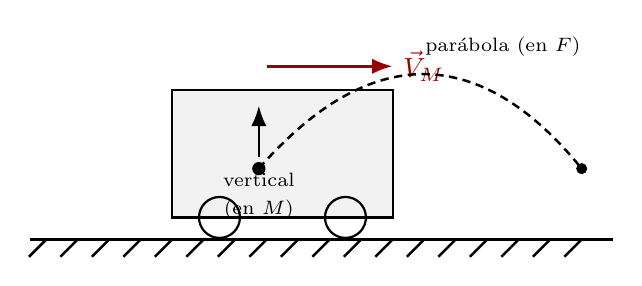
\begin{tikzpicture}[line width=0.9pt,>={Latex[length=2.6mm]}]
  \draw[thick] (0,0)--(7.4,0);
  \foreach \x in {0.2,0.6,...,7.2} \draw (\x,0)--(\x-0.22,-0.22);
  % vagon
  \draw[thick,fill=black!5] (1.8,0.28) rectangle (4.6,1.9);
  \draw[thick] (2.4,0.28) circle(0.26); \draw[thick] (4.0,0.28) circle(0.26);
  \draw[->,red!60!black,line width=1.1pt] (3.0,2.2)--(4.6,2.2) node[right]{$\vec V_M$};
  % pelota sube vertical dentro
  \fill (2.9,0.9) circle(2.4pt);
  \draw[->] (2.9,1.05)--(2.9,1.7) node[above]{};
  \node[align=center] at (2.9,0.55){\scriptsize vertical\\[-2pt]\scriptsize (en $M$)};
  % parabola en F (anden)
  \draw[densely dashed] (2.9,0.9) .. controls (4.3,2.5) and (5.7,2.5) .. (7.0,0.9);
  \fill (7.0,0.9) circle(2.0pt);
  \node at (6.0,2.45){\scriptsize parábola (en $F$)};
\end{tikzpicture}
\end{document}
